% =====================================================================
%  Chapter 5 -- Discussion
%  Structure follows Kwon (2025): interpretation of results, validity and
%  limitations, relevance to the field.
% =====================================================================
\chapter{Discussion}
\label{sec:discussion}

This chapter interprets the results of \cref{ch:results} against the two
research questions. The thermal performance and pumping power of the Galinstan
loop are discussed first (RQ1), followed by the inductor experiment (RQ2). The
validity and limitations of the measurements and models are then considered,
and finally the relevance of the findings to the cooling of PECs.

% ---------------------------------------------------------------------
\section{Interpretation of Results}
\label{sec:disc-interpretation}

\subsection{Thermal Performance of Galinstan in the Tested Cold Plate}
\label{sec:disc-performance}

The results in \cref{sec:results-measured} show that, at the flow rates
achieved, the Galinstan loop cooled the resistors less effectively than the
water loop, with a total thermal resistance 1.8 to 3.1 times higher
(\cref{tab:measured-performance}). However, the Galinstan tests ran at
\SIrange{0.8}{1.5}{\milli\litre\per\second}, one to two orders of magnitude below
the water tests (\SIrange{8.3}{58.3}{\milli\litre\per\second}). The comparison
therefore reflects the flow the MHD pump could deliver rather than a general
disadvantage of Galinstan as a coolant.

The reason lies in the limiting regime of the cold plate. Galinstan's NTU was 35
to 65 in the tests, so $\varepsilon \approx 1$ and $\Rcp \approx 1/(\mdot\,\cp)$.
The coolant therefore leaves the plate at almost the plate temperature, and heat
removal is limited by the ability of the flow to store and transport heat.
Galinstan's high thermal conductivity gives a wall heat transfer coefficient of
about \SI{7700}{\watt\per\metre\squared\per\kelvin}, roughly 7.5 times that of
laminar water (\cref{app:convection}). Its convective resistance $1/(hA)$ of
\SI{0.0085}{\celsius\per\watt} is lower than that of water even in turbulent
flow (\SIrange{0.012}{0.023}{\celsius\per\watt}). This advantage, however, is
not used in the current setup, because the convective term accounts for less
than \SI{3}{\percent} of Galinstan's $\Rcp$. Water, by contrast, has
$\NTU \approx 0.3$--0.4 at every tested flow, so convection makes up about
\SI{85}{\percent} of its $\Rcp$. These results support H1: Galinstan lowers the
convective resistance, but its low volumetric heat capacity and low flow rate
give a caloric resistance at least as large as the package resistance, so the
total resistance of the Galinstan loop is higher than that of the water loop.

\Cref{fig:disc-regimes}(a) extends this analysis over the full flow range.
Galinstan remains caloric-limited ($\NTU > 3$) over the whole laminar range and
up to about \SI{50}{\milli\litre\per\second}. Water, in contrast, stays close to
the convection-limited boundary above about \SI{10}{\milli\litre\per\second}.
For a caloric-limited coolant, the most important property is the volumetric
heat capacity $\rho\cp$, and here water has the advantage
(\cref{tab:disc-properties}): it absorbs about 1.8 times more heat per unit
volume per degree.

The same behaviour gives the Galinstan loop a much larger actuation range.
Because its cold plate is caloric-limited, its resistance follows the flow:
roughly halving the Galinstan flow, from 1.45 to
\SI{0.77}{\milli\litre\per\second}, raised the total resistance from 0.488 to
\SI{0.799}{\celsius\per\watt} (\cref{tab:measured-performance}). The
convection-limited water plate, in contrast, barely responded, with the total
resistance changing only from 0.257 to \SI{0.267}{\celsius\per\watt} over a
seven-fold change in flow. As discussed in \cref{sec:reliability}, the
flow rate of a single-phase loop is the control input used to suppress the
temperature swing of a component, part of the reliability requirement for PEC
thermal management (\cref{tab:cooling-strategies}). The pressure of an MHD pump
scales directly with its current (\cref{sec:em-pumping}), so the Galinstan loop
offers direct control over the component temperature through the pump current
across a wide range. In the tested water loop, changing the flow had almost no
effect on the resistor temperature. This range comes at the cost of a higher
resistance at the flows achieved here, but it is an advantage where the
temperature swing, rather than the peak temperature, limits component lifetime.

\begin{table}[htbp]
  \centering
  \caption{Coolant properties relevant to suitability. Thermal properties are
    those used in the model (\cref{tab:coolant-properties}).}
  \label{tab:disc-properties}
  \small
  \begin{tabularx}{\linewidth}{@{}lrrX@{}}
    \toprule
    Property & Galinstan & Water & Implication \\
    \midrule
    $\rho\cp$ (\si{\mega\joule\per\metre\cubed\per\kelvin})
      & 2.33 & 4.18 & Water carries 1.8$\times$ more heat per unit flow \\
    $k$ (\si{\watt\per\metre\per\kelvin}) & 16.5 & 0.60
      & Galinstan $h$ is about 27$\times$ higher at equal Nu \\
    $\mu$ (\si{\milli\pascal\second}) & 2.4 & 1.0
      & Laminar pressure drop 2.4$\times$ higher at equal flow \\
    $\rho$ (\si{\kilogram\per\metre\cubed}) & 6370 & 1000
      & 6.4$\times$ coolant mass for the same volume \\
    Pr & 0.053 & 6.97 & Heat diffuses far faster than momentum in Galinstan \\
    Electrical conductivity (\si{\siemens\per\metre})
      & $3.46 \times 10^{6}$~\cite{noauthor_gainsn_nodate} & $\ll 1$
      & Galinstan can be pumped electromagnetically, but heats and is retarded
        in AC fields \\
    Liquid range at \SI{1}{atm} (\si{\celsius})
      & 10 to $>1300$~\cite{noauthor_gainsn_nodate,hodes_potential_2014}
      & 0 to 100 & Galinstan cannot boil at component temperatures \\
    \bottomrule
  \end{tabularx}
\end{table}
\edited{\Cref{tab:disc-properties}: citations added for the electrical
conductivity and liquid range, matching \cref{tab:galinstan-properties}. The
lower end of the liquid range was $-19$; it is now \SI{10}{\celsius}, the
melting point of the grade used in this work (\cref{tab:galinstan-properties}).}

\begin{figure}[htbp]
  \centering
  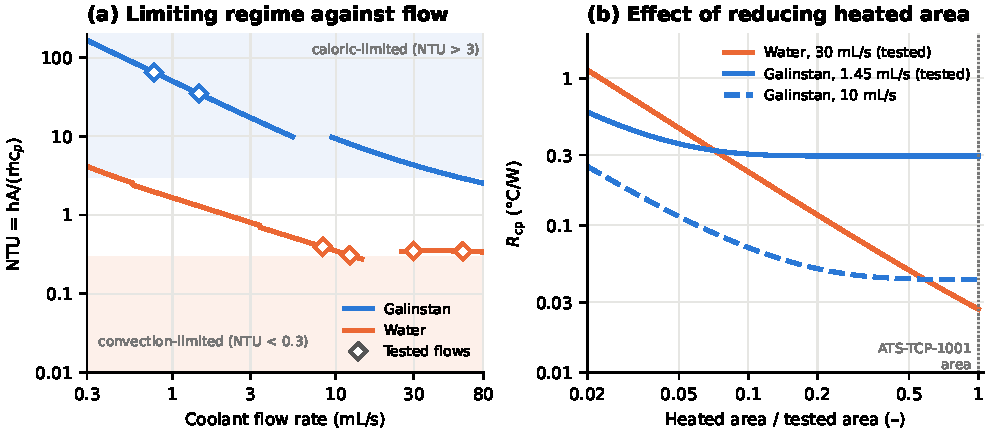
\includegraphics[width=\textwidth]{discussion_regimes.pdf}
  \caption{(a) NTU against flow rate for both coolants in the ATS-TCP-1001 cold
    plate, with the tested flows marked. Galinstan remains caloric-limited over
    the laminar range; water sits near the convection-limited boundary. Gaps
    mark the transitional range ($2300 < \mathrm{Re} < 4000$); turbulent
    Galinstan uses the Seban--Shimazaki correlation~\cite{bergman_fundamentals_2017}.
    (b) Indicative effect of reducing the heated area at fixed flow, with $h$
    held at its tested-geometry value. Water's $\Rcp$ rises in proportion to
    $1/A$, while Galinstan's at the tested flow is almost unaffected until the
    area falls to about a tenth of the tested value.}
  \label{fig:disc-regimes}
\end{figure}

\subsection{Pumping Power and Scalability}
\label{sec:disc-pumping}

RQ1 also asks how the pumping power of the two loops compares. At full flow, the
MHD pump drew \SI{0.85}{\watt}, about \SI{7}{\percent} of the \SI{11.5}{\watt}
drawn by the water pump, and it was more than 50 times smaller
(\cref{tab:pumps}). This is in line with An \emph{et al.}, who found that a
conduction pump drew less than \SI{15}{\percent} of the power of a mechanical
water pump for the same cooling performance~\cite{an_liquid_2024}, although here
the Galinstan loop also cooled less effectively. Per watt of pump power, the
Galinstan loop handled more heat, with a maximum coefficient of performance
(COP) of 200 against 47.6 for water. The low power draw does not, however,
reflect an efficient pump. The maximum mechanical efficiency of the MHD pump,
\SI{0.56}{\percent},
is an order of magnitude below the \SIrange{6}{10}{\percent} reported for DC
conduction pumps~\cite{an_liquid_2024,hodes_potential_2014}
(\cref{sec:em-pumping}), and far below the \SI{28.7}{\percent} of the
centrifugal water pump. Almost all of its input power is therefore dissipated
rather than delivered to the flow, which leaves considerable scope for a
redesigned pump. Fan \emph{et al.} show what is achievable: by reducing the
pressure drop of their loops to about one sixth with optimised connections and
cold plates, their MHD pumps reached flows of up to about
\SI{10}{\milli\litre\per\second} for less than
\SI{0.1}{\watt}~\cite{fan_liquid_2021,fan_high_2023} (\cref{tab:fan-comparison}). It is worth noting that the MHD pump was already at the
\SI{18}{\ampere} limit of its supply at full flow, so the Galinstan loop could
not be run at a higher flow.

For scalability, the more important question is the flow Galinstan would need
to match water. Because the cold plate is caloric-limited, the Galinstan $\Rcp$
is almost inversely proportional to the flow rate, as the simulations confirm up
to \SI{5}{\milli\litre\per\second} (\cref{fig:galinstan_rcp_cfd}). To match the
heat-capacity rate of
water at \SI{29.2}{\milli\litre\per\second} (\SI{122.0}{\watt\per\kelvin}),
Galinstan would need about \SI{52}{\milli\litre\per\second}, around 36 times the
full flow achieved here. The pressure of a DC conduction pump scales with current,
as shown by \cref{eq:mhd-pressure}, and the existing pump delivered
\SI{1.4}{\milli\litre\per\second} at the \SI{18}{\ampere} limit of its supply.
An increase in flow of this size would therefore require a redesigned pump
rather than simply a higher current. At equal volumetric flow, Galinstan also
needs about 2.4 times the pressure of water in laminar flow because of its higher
viscosity, and its density is 6.4 times that of water, which adds weight to the
loop (\cref{tab:disc-properties}). A comparison at equal pumping power, rather
than at the flow each pump could deliver, would therefore penalise Galinstan
further.

\subsection{Inductor Cooling and Eddy-Current Loss}
\label{sec:disc-inductor}

RQ2 asks whether the Galinstan loop can cool a power-dense inductor while adding
minimal loss, and how large the eddy-current loss induced in the coolant is. The
inductor was operated at an estimated loss of \SI{42.76}{\watt}, more than twice
the \SI{17.88}{\watt} datasheet loss limit above which its core requires active
cooling (\cref{sec:analytical-design}). Its maximum surface temperature was about
\SI{83}{\celsius} (\cref{fig:inductor-cam}), which shows that the Galinstan
loop can cool a power-dense inductor operating well beyond the loss its core
can dissipate without active cooling. The cooling effect of the plate is clear
from the steady-state thermal images: the upper core, which relies on natural
convection, ran markedly hotter than the lower core, which sits on the cold
plate (\cref{fig:inductor-cam-a}). This supports the first part of H2, that the
Galinstan loop cools the inductor beyond natural convection. The same difference
shows that the single-sided cold plate leaves part of the inductor's loss to be
removed by convection, and cooling both cores, as in the inductor of Gao
\emph{et al.}~\cite{gao_modeling_2022}, would make better use of the coolant.

The eddy-current measurements support the second part of H2. Placing the
inductor on the cold plate added \SI{11.7}{\milli\ohm} to the winding
resistance, whereas filling the plate with Galinstan added only
\SI{1.0}{\milli\ohm}, less than a tenth of the plate's own contribution. As
argued in H2,
the metal of the cold plate between the inductor and the
coolant is several skin depths thick at \SI{85}{\kilo\hertz}, so it shields the
Galinstan from the leakage field. Unshielded Galinstan is far more exposed: its
own skin depth at this frequency is about \SI{0.9}{\milli\metre} (for
$\sigma = \SI{3.46e6}{\siemens\per\metre}$~\cite{noauthor_gainsn_nodate}),
comparable to practical channel dimensions. The vial of Galinstan outside the
plate added \SI{10.3}{\milli\ohm}, an order of magnitude more than the coolant
inside the plate, although its volume and position differ. This agrees with the
initial ANSYS simulation, which found that \SI{1}{\milli\metre} of copper
shielding reduced the eddy-current loss in the coolant by more than
\SI{70}{\percent} (\cref{sec:inductor-design}). Without the plate, the effect of
the vial also fell with distance, from \SI{9.0}{\milli\ohm} at
\SI{1}{\centi\metre} to \SI{2.15}{\milli\ohm} beyond \SI{4}{\centi\metre}
(\cref{fig:rac_distance}), so keeping unshielded coolant a few centimetres from
the magnetics also limits the loss. Finally, the coolant flow did not change
measurably when the inductor was energised, which supports the final part of
H2.

% ---------------------------------------------------------------------
\section{Validity and Limitations}
\label{sec:disc-validity}

The steady-state data collected in this study are consistent across the two
loops and with the thermal models, but the conclusions rest on two Galinstan
tests and four water tests, and their limitations should be weighed. Four points
stand out.

First, the low-flow water results are limited by the flow measurement rather
than by the model. The measured $\Tres - \Tin$ stays between
\SI{16.1}{\celsius} and \SI{16.6}{\celsius} from
\SIrange{58.3}{8.3}{\milli\litre\per\second}, and the measured $\Rcp$ of
\SI{0.025}{\celsius\per\watt} at \SI{0.5}{\litre\per\minute} lies below water's
caloric limit $1/(\mdot\,\cp)$ of \SI{0.029}{\celsius\per\watt} at the indicated
flow (\cref{fig:water_rcp}). A cold plate cannot have $\Rcp < 1/(\mdot\,\cp)$, so
the true flow in that test must have been at least
\SI{9.6}{\milli\litre\per\second}, about \SI{15}{\percent} above the reading.
This supports the conclusion that the flow meter under-reads below its rated
range. It is also likely that these tests were not truly laminar. With the water
viscosity of about \SI{0.75}{\milli\pascal\second} at the \SI{33}{\celsius} test
temperature, the \SI{0.73}{\litre\per\minute} test reaches
$\mathrm{Re} \approx 2600$, in the transitional range, and any under-reading of
the flow raises this further. Disturbances from the pump, the valve and the
U-bends can also persist in the short passes, where the thermal entry length far
exceeds the pass length. If these tests are treated as turbulent, the datasheet
trend predicts $\Tres$ within \SI{0.7}{\celsius}, so the laminar
predictions in \cref{tab:tn_results} are best read as a conservative upper
bound.

Second, $\Rpack$ was calibrated on the turbulent water tests, where the plate is
close to isothermal. Galinstan's coolant temperature rise of
\SIrange{17}{18}{\celsius} violates this assumption: the outlet end of the plate
runs hotter than the mean, and the $\Rpack$ inferred for Galinstan ranges from
\SIrange{0.19}{0.24}{\celsius\per\watt} for an isothermal plate to
\SIrange{0.33}{0.51}{\celsius\per\watt} for uniform heat flux. The full-flow
Galinstan point lying slightly below its caloric limit (\cref{fig:galinstan_rcp})
is consistent with this. The Galinstan flow itself also relies on a small EMF,
which is less accurate at lower pump current, although it agreed with the energy
balance to within \SI{4}{\percent}. The lumped model therefore describes
Galinstan less reliably than water, although its prediction of the Galinstan
resistor temperatures to within \SI{2.5}{\celsius} (\cref{sec:results-tn})
shows that it captures the dominant behaviour.

Third, the conjugate heat transfer simulations address the main weakness of the
lumped model. They are mesh-independent above \num{427e3} cells and reproduce
all four probe temperatures within \SI{1.4}{\celsius} for both Galinstan tests.
The consistent over-prediction of the right-hand resistor by about
\SI{1.3}{\celsius} in both runs suggests a small systematic asymmetry in the
model, such as the heat-load distribution, rather than random error. For water,
the model under-predicts the resistor temperatures by about
\SIrange{2.3}{2.4}{\celsius}, which points to an over-predicted wall heat
transfer coefficient in the turbulent model (\cref{app:cht_validation}). The
model is therefore slightly pessimistic for Galinstan and optimistic for water,
so any advantage it shows for Galinstan is, if anything, understated. With this
in mind, the CHT model can be used with reasonable confidence to compare
geometries and flows that the test rig could not reach.

Fourth, the inductor experiment was run at a single operating point. Its heat
load is an estimate from the core-loss model and the measured winding
resistance, and the measured surface temperature of about \SI{83}{\celsius} is
above the \SI{65}{\celsius} assumed when the core loss was modelled, so the true
core loss will differ from the \SI{30.81}{\watt} estimate. The AC resistances
in \cref{fig:rac_configurations,fig:rac_distance} were measured at the
\SI{85}{\kilo\hertz} operating frequency, but each value comes from a single
measurement at low excitation, and the absolute resistance varied between
sessions, so only changes within a session are compared.

More generally, the study used a single cold plate designed for water, and the
coolants were compared at the flow each pump could deliver rather than at equal
pumping power. The water temperature rise across the plate was also below the
thermocouple accuracy, so the water energy balance could not be checked
independently.

% ---------------------------------------------------------------------
\section{Relevance to the Field}
\label{sec:disc-suitability}

The NTU analysis gives a clear criterion for where Galinstan is advantageous:
where the cooling surface, rather than the coolant flow, limits heat removal,
that is, where water would be convection-limited. \Cref{fig:disc-regimes}(b)
illustrates this using the $\varepsilon$--NTU model. The heated area is scaled
by a factor $f$ while the flow rate and heat transfer coefficient are held at
their values in the tested cold plate, so that $\NTU$ falls in proportion to $f$
and $\Rcp = 1/[\mdot\,\cp\,(1 - e^{-f\,\NTU_0})]$, where $\NTU_0$ is the value
for the full plate. This represents concentrating the same heat into a smaller
footprint or a shorter heated length, and the method and its assumptions are
given in \cref{app:area-scaling}. Reducing the heated area at fixed flow raises
water's $\Rcp$ almost in proportion, because water is already close to
convection-limited. At the tested flow, Galinstan's $\Rcp$ barely changes until
the area is reduced to about a tenth, because it simply uses up its excess
$hA$. At \SI{5}{\percent} of the tested area, Galinstan at
\SI{10}{\milli\litre\per\second} ($\Rcp \approx \SI{0.12}{\celsius\per\watt}$)
outperforms water at three times the flow
($\Rcp \approx \SI{0.46}{\celsius\per\watt}$). Galinstan's resistance only
begins to rise once $f\,\NTU_0$ falls to about 3, so a coolant that starts with a
large NTU can absorb a large reduction in area before its performance suffers.
Because $h$ is held fixed and pressure drop is not considered, the result is
indicative only, but it shows the type of application in which Galinstan's
conductivity becomes useful.
\edited{``About a fifth'' changed to ``about a tenth'': with $\NTU_0 = 34.9$ the
resistance starts to rise at $f \approx 3/\NTU_0 = 0.09$ (\cref{app:area-scaling}),
and \cref{tab:app-area} shows no change at $f = 0.2$. The caption of
\cref{fig:disc-regimes} was changed to match.}

Galinstan is therefore best suited to applications that combine (i)~high heat
flux over a small area, such as direct cooling of power semiconductors or local
hot spots, or minichannel and microchannel heat sinks; (ii)~a pump able to
deliver flow rates comparable to water, for which a sealed electromagnetic pump
with no moving parts may offer a reliability advantage; (iii)~component
temperatures near or above \SI{100}{\celsius}, where water would boil without
pressurisation; and (iv)~locations away from strong alternating magnetic fields,
or where the coolant is shielded from them by the cold plate, as in
\cref{sec:disc-inductor}.

In an IPT system, these criteria point to the power electronics, rather than the
pads, as the best place for Galinstan. In the \SI{10}{\kilo\watt} system of Kim
\emph{et al.}, the inverter and rectifier each dissipated about
\SIrange{70}{80}{\watt} in small switching devices placed away from the coupler,
where the heat flux is high and the magnetic field is weak
(\cref{sec:ipt-losses})~\cite{kim_thermal_2022}. The larger pad losses, by
contrast, are spread over about \SI{0.5}{\metre\squared} inside the strongest
alternating field at \SI{85}{\kilo\hertz}, so a cold plate under the pad would
see a low heat flux, for which water is adequate, together with a strong leakage
field. The inductor experiment shows that the leakage field need not rule
Galinstan out: coolant shielded by the metal of the cold plate added only
\SI{1.0}{\milli\ohm} to the winding resistance at \SI{85}{\kilo\hertz}, against
\SI{10.3}{\milli\ohm} for unshielded coolant beside the inductor
(\cref{sec:results-eddy}). Galinstan could therefore also cool compact
magnetics, such as the tank inductors and transformer, where heat is
concentrated in a small volume, provided the coolant is shielded.
\Cref{tab:disc-suitability} applies these criteria to the main components of an
IPT system.

\begin{table}[htbp]
  \centering
  \caption{Indicative suitability of Galinstan cooling for IPT system
    components, based on the criteria of \cref{sec:disc-suitability}.}
  \label{tab:disc-suitability}
  \small
  \begin{tabularx}{\linewidth}{@{}l>{\raggedright\arraybackslash}p{2.6cm}cX@{}}
    \toprule
    Component & Heat load character & Suitability & Reason \\
    \midrule
    Inverter and rectifier modules & High flux, small area & Good
      & Water likely convection-limited; much weaker AC fields than at the
        coupler \\
    Compact magnetics (tank inductors, transformer) & High flux, small volume
      & Possible
      & Leakage-field loss is small if the coolant is shielded by the cold
        plate (\cref{sec:results-eddy}) \\
    Coupler coils (Litz) and ferrite pads & Distributed, low flux & Limited
      & Large area, where water is adequate; strongest AC field, so the coolant
        must be shielded \\
    Resonant compensation capacitors & Moderate flux & Limited
      & Benefit only if close to their temperature limit; proximity to high
        voltage and AC fields \\
    Vehicle-side assembly & Weight-sensitive & Poor
      & 6.4$\times$ the coolant mass of water, and high material cost \\
    Large cold plates at low flow (as tested) & Low flux, large area & Poor
      & Caloric-limited; water carries 1.8$\times$ more heat per unit flow \\
    \bottomrule
  \end{tabularx}
\end{table}
\edited{\Cref{tab:disc-suitability}: coupler coils and pads changed from
``Poor'' to ``Limited'', since the eddy-current results show that a shielding
cold plate keeps the coolant's loss small, and a row added for compact magnetics,
which the inductor experiment represents.}

These findings agree with Hodes \emph{et al.}~\cite{hodes_potential_2014}, who
found that Galinstan's low volumetric heat capacity makes its caloric resistance
a larger share of the total than for water (\SI{55}{\percent} against
\SI{40}{\percent} in their optimised minichannel), and that its advantage depends
on geometries that exploit its high conductivity. The larger caloric share found
here (above \SI{97}{\percent}) reflects a cold plate designed for water and a
flow rate far below their optimum, rather than a contradiction of their result.
\issue{Check the volumetric heat-capacity ratio: Hodes quote 0.45, while the
properties used here give $2.33/4.18 = 0.56$; the difference is likely the
Galinstan $\cp$ (see the 360 vs \SI{366}{\joule\per\kilogram\per\kelvin} note).
\Cref{tab:galinstan-properties} also quotes 0.45.}

Despite the limitations above, the results show that a magnetohydrodynamically
pumped Galinstan loop can cool both a resistive load and a power-dense inductor,
and that the loss it adds near magnetics can be kept small when the coolant is
shielded by the cold plate. Its performance in the tested system is set by the
pump rather than by the coolant, so the case for liquid metal cooling in PECs
rests on higher-flow pumps and on cold plates designed to exploit its high
conductivity.

% ---------------------------------------------------------------------
\section{Recommendations for Further Work}
\label{sec:disc-limitations}

Further work should:
\begin{enumerate}
  \item compare the coolants at equal pumping power, using the CHT model to
    obtain the pressure drop as well as the temperature;
  \item test Galinstan at higher flow rates, closer to
    \SIrange{10}{30}{\milli\litre\per\second}, with an independently calibrated
    flow meter, which will require a redesigned pump;
  \item use the CHT model to evaluate small-area, high-flux geometries such as
    minichannel cold plates, where \cref{fig:disc-regimes}(b) indicates that
    Galinstan may outperform water;
  \item repeat the inductor test with the pump off and with the coolant
    unshielded, repeat the $R_{\mathrm{ac}}$ measurements to estimate their
    spread, and quantify eddy-current heating and MHD drag through coupled
    electromagnetic--thermal analysis before Galinstan is placed near an IPT
    coupler; and
  \item assess long-term material compatibility, since gallium alloys attack
    aluminium and copper requires protection at higher
    temperatures~\cite{an_liquid_2024}.
\end{enumerate}
